\section{Experiments}
The main comparisons use Astana data with the same local loss and training settings. A Singapore auxiliary experiment evaluates the prefix objective with complete local labels.

\subsection{Data and Time Definitions}
Astana\cite{astana2025} was released on Zenodo on June 29, 2025 under CC BY 4.0, with data collected on three bus routes during July--September 2024. The interval records used here span July 29--September 21, 2024 and contain 785,976 records from 19,769 trips. Preprocessing requires a continuous directed stop chain, running times of 5--1,800 seconds, and dwell times of 0--900 seconds. Trips violating these conditions are removed in full. The resulting sample contains 10,910 trips, 439,659 intervals, and 586 directed interval identities. The longest valid trip has 55 intervals, which sets the padding length; longer trips are not truncated.

Interval identities combine direction and endpoint stop identifiers. Targets use the recorded running-time field, and their sum supplies the input total, excluding dwell. Trips are ordered chronologically and split 60\%/20\%/20\%. From the first 60\%, 5,891 trips are used for fitting and 655 for checkpoint selection; the middle 20\% (2,182 trips) is the development evaluation set. The final 20\% is excluded from the reported results (Table~\ref{tab:partitions}).
\begin{table}[t]
\centering\footnotesize
\caption{Astana partitions and valid-label populations.}\label{tab:partitions}
\begin{tabular}{lrr}\toprule
Role & Trips & Intervals\\\midrule
Model fitting & 5,891 & 237,203\\
Checkpoint selection & 655 & 26,561\\
Development evaluation & 2,182 & 87,715\\
\bottomrule\end{tabular}
\end{table}

Models use 31 geometry, route, stop, and departure-calendar features. Normalization is estimated from fitting features only. Inputs exclude target-derived statistics, actual interval entry times, label-quality fields, and additional historical targets.

The Singapore auxiliary collection spans May 5--June 19, 2017. Interval targets are differences between timestamp midpoints of consecutive observed stop runs; dwell is not independently removed. Each source record contributes its longest valid contiguous fragment, requiring at least eight intervals, durations of 30--1,800 seconds, and chord speed below 25 m/s. The maximum length is 87; no interpolation or cross-record stitching is used. Training covers May 5--June 5, checkpoint selection June 6--8, and development evaluation June 10--16, with a one-day gap. We use 50,000, 5,000, and 10,000 trips respectively, including 197,301 development intervals. Because the target definition differs from Astana, these results are reported separately.

\subsection{Label Budgets and Training Settings}
Training and validation use the same label percentage, with budgets of 1\%, 5\%, and 10\%. Training exposes 2,372, 11,860, and 23,720 labels respectively; validation exposes 265, 1,328, and 2,656. Valid positions are randomly permuted and sampled using three nested layouts. Each layout is trained with three independent initializations, giving nine runs per neural method and budget. Paired methods share initial states, batches, and visible labels; hidden targets are masked before training and validation.

The encoder has width 64, two Transformer layers, four heads, feed-forward width 256, and zero dropout. The primary Ours/direct comparisons use AdamW with initial learning rate 0.001, cosine decay, 960 updates, and checkpoint selection every 24 updates. The validation-selected correction bounds are $\rho=0.10$, 0.05, and 0.25 for the 1\%, 5\%, and 10\% budgets. Coverage and mechanism controls use a separate 240-update protocol with AdamW learning rate 0.003, weight decay $10^{-4}$, gradient clipping at 5, and batches of 256 trips cycled through a random permutation. Calendar/correction and correction-parameterization ablations use three 10\% label layouts and three paired initializations per layout; interval-count controls use one layout and three initializations. Development metrics use all local labels in the development evaluation set.

Singapore uses complete training and checkpoint-selection labels, batches of 2,048, and the same network and optimizer settings. Auxiliary local weights are
\begin{equation}
w_{qi}=1+0.75\frac{t_{qi}}{\max(\bar t_q,1)}
+1.5\min\left(\frac{(t_{qi}-180)_+}{180},5\right),
\end{equation}
where $\bar t_q$ is the valid mean duration. We normalize by the valid weight sum and use prefix coefficient 0.35. These objectives require complete labels and are confined to the auxiliary experiment. Additional-history conditions are reported separately in the supplement.

\subsection{Baselines and Metrics}
Uniform allocation assigns $T_q/L_q$ per interval. Segment means pool visible training labels for each interval, use the global visible-label mean for unsupported intervals, and rescale to the total. NNLS-Ridge fits nonnegative identity coefficients by
\begin{align}
\min_{\boldsymbol v\geq0}\quad&
\frac{\|C\boldsymbol v-\boldsymbol T\|_2^2}{N_F}
+\frac{\lambda}{S}\|\boldsymbol v\|_2^2\nonumber\\
&+\frac{\alpha}{N_V}\sum_{(q,i)\in V}(v_{s_{qi}}-t_{qi})^2,
\label{eq:inverse}
\end{align}
where $C$ counts intervals in trips; $N_F$, $N_V$, and $S$ count training trips, visible labels, and identities. Ten candidates combine $\lambda\in\{0.01,1\}$ and $\alpha\in\{0,1,10,100,1000\}$, selected using the same limited validation labels. Predictions are rescaled to the total. This baseline tests nonnegative aggregate inversion without context.

Direct prediction uses the same features and sequence backbone, with local log-duration and route-ratio mappings followed by identical total rescaling. It omits the base-plus-correction structure. Both methods instantiate the same parameters and share initial states; their actual computation and gradient paths depend on the prediction form. The author-code ProbETA adaptation\cite{xu2025probeta} trains on visible singleton Gaussian likelihoods and obtains a conditional nonnegative solution given the total. Its inputs and loss differ, so its results and training-budget checks are reported separately.

MAE and RMSE are microaveraged over valid intervals; $\mathrm{WAPE}(\%)=100\sum|\hat t-t|/\sum_qT_q$. Prefix50 averages absolute cumulative error at $\lceil L_q/2\rceil$ over trips. Top-10\% MAE scores each trip's $\lceil0.1L_q\rceil$ largest true intervals. Long intervals have true duration at least 300 seconds. Labels define evaluation groups only.

Tables report mean errors and sample standard deviations across runs. The final chronological split remains unopened.

\subsection{Overall Results}
\begin{table*}[t]
\centering\scriptsize\setlength{\tabcolsep}{2.5pt}
\caption{Astana development-set errors on 2,182 trips and 87,715 intervals. Values are mean $\pm$ sample SD except the deterministic uniform reference. Neural methods and the fixed-weight combination use nine runs; identity and NNLS use three label layouts; ExtraTrees uses three layouts.}\label{tab:limited}
\begin{tabular}{llrrrrrr}\toprule
Budget & Method & MAE & RMSE & WAPE (\%) & Prefix50 & Top-10\% MAE & Long MAE\\\midrule
1\% & Uniform & $54.28$ & $87.17$ & $58.54$ & $276.78$ & $182.45$ & $338.02$\\
1\% & Identity means & $\mathbf{31.50\pm0.56}$ & $59.24\pm0.88$ & $\mathbf{33.96\pm0.61}$ & $159.41\pm4.72$ & $92.90\pm1.13$ & $172.37\pm6.11$\\
1\% & NNLS-Ridge & $32.15\pm0.58$ & $60.95\pm0.78$ & $34.67\pm0.63$ & $167.09\pm6.76$ & $93.62\pm0.93$ & $\mathbf{172.18\pm6.20}$\\
1\% & ExtraTrees & $32.47\pm0.12$ & $61.95\pm0.58$ & $35.01\pm0.13$ & $161.53\pm3.92$ & $98.80\pm0.93$ & $184.85\pm3.94$\\
1\% & Direct prediction & $33.19\pm0.60$ & $60.34\pm0.86$ & $35.79\pm0.65$ & $157.99\pm4.73$ & $95.17\pm2.30$ & $177.43\pm5.68$\\
1\% & Ours & $32.61\pm0.28$ & $60.68\pm0.62$ & $35.16\pm0.30$ & $156.04\pm4.48$ & $95.69\pm2.65$ & $183.25\pm7.16$\\
1\% & Ours + Direct ($\alpha=0.5$) & $31.79\pm0.26$ & $\mathbf{58.80\pm0.50}$ & $34.27\pm0.28$ & $\mathbf{151.72\pm5.06}$ & $\mathbf{92.83\pm2.23}$ & $177.33\pm6.24$\\
\midrule
5\% & Uniform & $54.28$ & $87.17$ & $58.54$ & $276.78$ & $182.45$ & $338.02$\\
5\% & Identity means & $29.99\pm0.06$ & $56.97\pm0.10$ & $32.34\pm0.06$ & $156.07\pm2.84$ & $88.98\pm0.92$ & $169.82\pm4.07$\\
5\% & NNLS-Ridge & $30.43\pm0.05$ & $58.06\pm0.13$ & $32.81\pm0.06$ & $163.04\pm3.70$ & $89.55\pm0.87$ & $170.01\pm4.06$\\
5\% & ExtraTrees & $29.70\pm0.30$ & $58.17\pm0.97$ & $32.02\pm0.32$ & $147.19\pm2.76$ & $92.60\pm1.79$ & $181.86\pm4.64$\\
5\% & Direct prediction & $29.46\pm0.33$ & $56.12\pm0.91$ & $31.76\pm0.36$ & $148.30\pm4.96$ & $87.44\pm2.33$ & $\mathbf{164.37\pm7.44}$\\
5\% & Ours & $29.38\pm0.13$ & $57.05\pm0.38$ & $31.68\pm0.14$ & $148.35\pm2.44$ & $88.32\pm1.53$ & $171.22\pm4.06$\\
5\% & Ours + Direct ($\alpha=0.5$) & $\mathbf{28.78\pm0.16}$ & $\mathbf{55.47\pm0.46}$ & $\mathbf{31.04\pm0.17}$ & $\mathbf{145.18\pm2.71}$ & $\mathbf{86.13\pm1.72}$ & $165.47\pm5.79$\\
\midrule
10\% & Uniform & $54.28$ & $87.17$ & $58.54$ & $276.78$ & $182.45$ & $338.02$\\
10\% & Identity means & $29.85\pm0.10$ & $56.86\pm0.50$ & $32.19\pm0.10$ & $155.72\pm1.10$ & $88.54\pm0.10$ & $170.86\pm3.21$\\
10\% & NNLS-Ridge & $30.21\pm0.05$ & $57.57\pm0.61$ & $32.58\pm0.05$ & $162.35\pm1.72$ & $88.89\pm0.11$ & $170.88\pm3.23$\\
10\% & ExtraTrees & $29.03\pm0.18$ & $56.70\pm0.53$ & $31.30\pm0.19$ & $141.88\pm2.10$ & $89.96\pm1.21$ & $176.56\pm3.97$\\
10\% & Direct prediction & $28.48\pm0.14$ & $54.63\pm0.76$ & $30.71\pm0.15$ & $143.01\pm4.08$ & $83.64\pm1.03$ & $\mathbf{157.80\pm3.62}$\\
10\% & Ours & $28.78\pm0.16$ & $55.52\pm0.32$ & $31.03\pm0.17$ & $144.64\pm2.40$ & $85.50\pm0.67$ & $166.07\pm3.30$\\
10\% & Ours + Direct ($\alpha=0.5$) & $\mathbf{28.06\pm0.10}$ & $\mathbf{53.99\pm0.34}$ & $\mathbf{30.26\pm0.11}$ & $\mathbf{140.84\pm2.59}$ & $\mathbf{82.87\pm0.61}$ & $159.39\pm3.30$\\
\bottomrule\end{tabular}
\end{table*}

\begin{table}[t]
\centering\footnotesize\setlength{\tabcolsep}{3pt}
\caption{Paired Ours-minus-direct MAE across the same three label layouts and three initializations. Negative differences favor Ours; SD is across nine paired runs.}\label{tab:paired}
\begin{tabular}{lrrr}\toprule
Budget & Mean difference (s) & SD (s) & Ours wins\\\midrule
1\% & -0.579 & 0.624 & 8/9\\
5\% & -0.075 & 0.353 & 6/9\\
10\% & +0.295 & 0.169 & 0/9\\
\bottomrule\end{tabular}
\end{table}

Each neural method has nine paired runs per label budget, sharing the three label layouts and three initializations. ExtraTrees selects minimum leaf sizes 2, 8, and 8 using validation data and is evaluated on the three layouts. Identity means and NNLS-Ridge are fitted separately at each label budget. The fixed-weight Ours+Direct row is a validation-selected ensemble ($\alpha=0.5$), not the Ours model alone.

At 1\%, identity means have the lowest MAE (31.498 s); Ours reaches 32.607 s and direct prediction 33.186 s. At 5\%, Ours (29.383 s) is 0.075 s below direct prediction (29.457 s), with six of nine paired runs favoring Ours; the ensemble gives 28.783 s. At 10\%, Ours (28.776 s) is 0.295 s above direct prediction (28.481 s), and none of the nine paired runs favor Ours; the ensemble gives 28.065 s. The ensemble has the lowest mean MAE at 5\% and 10\%, but identity means remain better at 1\%; long-interval MAE also remains higher for Ours at all three budgets. These development results do not establish a uniform advantage for Ours across budgets or metrics.

Fig.~\ref{fig:comparison} reports layout-level MAE differences from direct prediction. Ours is lower in eight of nine paired runs at 1\%, six at 5\%, and none at 10\% (Table~\ref{tab:paired}). The plotted points aggregate the three initializations within each layout for neural methods; the error bars show sample standard deviation across the three layouts. This visualization summarizes development comparisons and does not provide an independent test estimate.

Across all three budgets, Ours has higher long-interval MAE than direct prediction (Table~\ref{tab:limited}), despite exact total conservation. Errors in a few long intervals can therefore remain hidden by an accurate trip sum.

\begin{figure*}[t]
\centering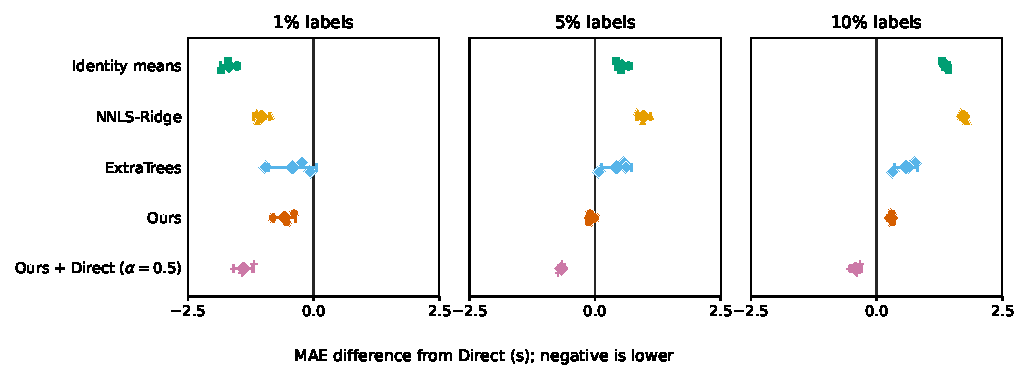
\includegraphics[width=\textwidth]{figures/followup_mae_differences.pdf}
\caption{Development-set MAE difference from direct prediction across three label layouts. Negative values indicate lower MAE. Neural results average three paired initializations within each layout; identity means and NNLS use the mean direct score for each layout, while ExtraTrees uses the paired seed-42 direct run. Points show layouts and horizontal bars show the across-layout mean and sample standard deviation.}
\label{fig:comparison}
\end{figure*}

\subsection{Label Quantity and Coverage}
Label budgets change the amount of information available for learning, but equal counts can cover different intervals. In a layout experiment with complete validation labels, restricting 23,720 training labels to the first 20\% of each trip reduces observed identities from 301 to 115 and raises our method's MAE from 28.522 to 50.121 seconds. A moving 40\% blackout retains 310 identities and gives 28.774 seconds. Prefix placement changes both positions and interval coverage, so the original comparison cannot identify position's independent effect. Full results are reported in the supplement.

\begin{table*}[t]
\centering\footnotesize\setlength{\tabcolsep}{4pt}
\caption{Label-placement control with identical identity-specific label counts; three initializations and limited validation labels. Errors in seconds. Bold marks the lowest error within each comparable group.}\label{tab:controlled_coverage}
\begin{tabular}{llrr}\toprule
Layout & Method & MAE & Prefix50\\\midrule
First 20\% & Ours & $\mathbf{50.121\pm0.938}$ & $\mathbf{318.01}$\\
First 20\% & Direct prediction & $50.472\pm0.549$ & $326.46$\\
Identity-matched random & Ours & $\mathbf{50.397\pm0.816}$ & $\mathbf{348.30}$\\
Identity-matched random & Direct prediction & $51.374\pm0.609$ & $362.85$\\
\bottomrule\end{tabular}
\end{table*}

To distinguish these changes, we use the main experiment's limited validation labels, fix the first-20\% layout, and count labels for each of its 115 intervals. A random training layout then draws \emph{exactly the same count for every interval}, totaling 23,720. Methods share validation labels, initial states, and batches. The layouts have identical interval sets and counts, while the labels occupy different trip positions.

Our method gives MAE of 50.121 seconds under prefix placement and 50.397 under matched random placement; direct prediction gives 50.472 and 51.374 (Table~\ref{tab:controlled_coverage}). Randomizing positions does not recover the roughly 29-second error with broader interval coverage, weakening an explanation that attributes all deterioration to early placement. This control uses one layout, does not fully balance trips and contexts, and selects the final update in all three matched-random fits. These results do not identify coverage's contribution independently of position.

\subsection{Correction Mechanisms and Ablations}
\begin{table*}[t]
\centering\footnotesize\setlength{\tabcolsep}{4pt}
\caption{Correction controls under a separate fixed-$\rho=0.45$, 240-update protocol across three 10\% layouts and three paired initializations per layout. Errors in seconds; mean $\pm$ sample SD. Uncentered scaling also changes effective amplitude. Bold marks the lowest error within each comparable group.}\label{tab:redistribution}
\begin{tabular}{llrrr}\toprule
Variant & $\rho$ & MAE & RMSE & Prefix50\\\midrule
Weighted centering & 0.10 & $28.849\pm0.189$ & $56.063\pm0.328$ & $145.34$\\
Weighted centering & 0.25 & $28.677\pm0.184$ & $55.503\pm0.353$ & $\mathbf{143.64}$\\
Weighted centering (fixed-$\rho$ control) & 0.45 & $28.633\pm0.239$ & $\mathbf{54.930\pm0.401}$ & $145.26$\\
Without weighted centering & 0.45 & $\mathbf{28.632\pm0.218}$ & $55.030\pm0.227$ & $143.94$\\
\bottomrule\end{tabular}
\end{table*}

We compare correction amplitudes and weighted centering under a separate fixed-$\rho=0.45$, 240-update protocol across three 10\% training/validation layouts and three paired initializations per layout (Table~\ref{tab:redistribution}). With weighted centering, $\rho=0.10$, 0.25, and 0.45 give MAE of 28.849, 28.677, and 28.633 seconds; their RMSE values are 56.063, 55.503, and 54.930 seconds. The 0.25 setting has the lowest Prefix50, so no amplitude leads on every metric. These controls are separate from the validation-selected, 960-update main comparison.

Removing weighted centering from Eq.~\eqref{eq:redistribution}, setting $r_i=b_i+\rho b_i\tanh z_i$, and applying the same total rescaling gives the following output. For $m=\sum_jp_j\tanh z_j$,
\begin{equation}
\hat t_i^{\mathrm{unc}}=T p_i\left[1+\frac{\rho(\tanh z_i-m)}{1+\rho m}\right].
\end{equation}
Compared with Eq.~\eqref{eq:shape}, rescaling also changes the effective correction amplitude. This comparison therefore tests two parameterizations without isolating centering's effect. The uncentered variant has MAE 28.632 seconds, effectively tied with the fixed-$\rho=0.45$ centered control at 28.633 seconds. Paired differences in Fig.~\ref{fig:ablation}(b)--(d) vary across metrics and runs, and these results do not establish an accuracy benefit from weighted zero-sum centering. It preserves the sum of the base estimates, while local accuracy still depends on the learned allocation.

\begin{table}[t]
\centering\footnotesize\setlength{\tabcolsep}{4pt}
\caption{Ablations with one 10\% training/validation mask and three initializations. Errors in seconds. Bold marks the lowest error within each comparable group.}\label{tab:finite_ablation}
\begin{tabular}{lrr}\toprule
Variant & MAE & Prefix50\\\midrule
Ours & $28.709\pm0.396$ & $\mathbf{144.27}$\\
No correction & $29.011\pm0.170$ & $144.66$\\
No calendar & $\mathbf{28.588\pm0.132}$ & $148.43$\\
Shuffled calendar & $29.033\pm0.153$ & $151.04$\\
\bottomrule\end{tabular}
\end{table}

Table~\ref{tab:finite_ablation} summarizes nine outcomes per condition across three 10\% training/validation layouts and three paired initializations per layout. Removing trip correction raises MAE from 28.633 to 29.038 seconds in all nine paired comparisons. Correction improves the base estimate within the same model, but this ablation does not establish an advantage of the complete method over direct prediction.

Joint calendar shuffling preserves feature combinations within each partition but breaks their association with trips; MAE rises to 29.010 seconds, with higher error than the primary model in all nine paired comparisons. Removing calendar fields gives a slightly lower mean MAE of 28.570 seconds, although RMSE and Prefix50 are higher. Mismatched information and missing information therefore have different effects, and these results do not establish that calendar features are indispensable. Both branches receive calendar context, and correction gains cannot be attributed entirely to one temporal factor.

The Singapore auxiliary experiment compares prefix-loss normalization with complete labels. Our method gives MAE of 19.518 seconds when normalization includes padding, 19.445 when it counts valid positions, and 19.490 without the prefix objective; direct prediction with valid-position normalization gives 19.545. The valid-position variant is slightly better than direct prediction and no-prefix fitting in all three pairs, but has higher long-interval error than the padding-inclusive variant. Overall and long-interval errors change differently; this complete-label experiment also differs from sparse Astana supervision.

\begin{figure}[t]
\centering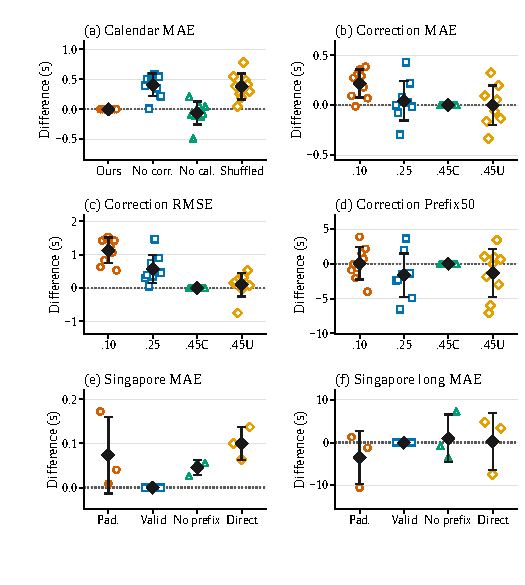
\includegraphics[width=\columnwidth]{figures/ablation_panels.pdf}
\caption{Paired error differences; positive values indicate increased error. References are Ours in (a), weighted centering with $\rho=0.45$ in (b)--(d), and valid-position prefix normalization in (e)--(f). Open markers show paired runs; filled diamonds and error bars show the mean and sample standard deviation (nine pairs per Astana condition, three per Singapore condition).}
\label{fig:ablation}
\end{figure}

\subsection{Interval Cases and Efficiency}
\begin{figure}[t]
\centering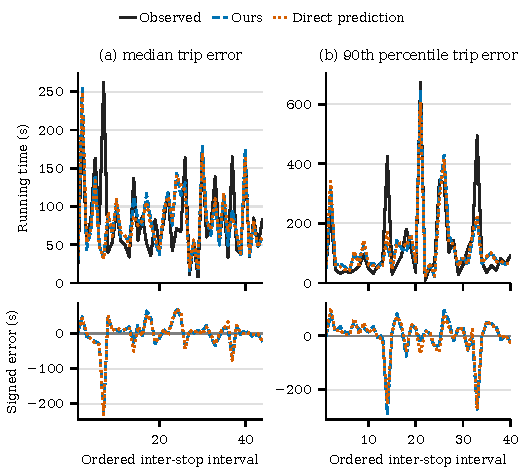
\includegraphics[width=\columnwidth]{figures/local_cases.pdf}
\caption{Development-trip interval times and signed errors. Cases nearest the median and 90th percentile of Ours trip MAE are selected from one paired run at 10\% labels. Black, blue, and orange curves show truth, Ours, and direct prediction, respectively.}\label{fig:cases}
\end{figure}
Fig.~\ref{fig:cases} shows local errors under the same total. The selected trips contain 44 and 40 intervals; their Ours/direct MAE values are 25.997/26.486 and 43.178/43.521 seconds. The larger errors are compensated by other intervals, so exact total conservation does not ensure an accurate local profile.

Timing uses the same RTX 4090 D, float32, and 256-trip batches, with ten warmups and 30 synchronized measurements. Both methods instantiate 195,079 parameters with different computation paths. The supplement reports median forward latency and interquartile ranges. Measurements include network computation and total rescaling but exclude input loading and host transfer.

\subsection{Additional Evaluation}
\begin{table*}[t]
\centering\footnotesize\setlength{\tabcolsep}{6pt}
\caption{Singapore complete-label comparison on 14,933 OD trips and 295,318 intervals. Methods without historical inputs share the supplied OD total; the strict-past reference has additional earlier-trip labels. Errors are in seconds; learned methods report mean $\pm$ population standard deviation over three runs. Bold marks the lowest error in the group without historical inputs.}
\label{tab:singapore-common-visible}
\begin{tabular}{lrrrr}
\toprule
Method & Runs & MAE (s) & RMSE (s) & Prefix50 (s)\\
\midrule
\multicolumn{5}{l}{\textit{Common-visible methods}}\\
Ours (complete labels) & 3 & $\mathbf{19.286\pm0.033}$ & $\mathbf{28.009\pm0.070}$ & $\mathbf{54.938\pm1.043}$\\
MixTTE adapter & 3 & $25.760\pm0.053$ & $35.654\pm0.171$ & $66.292\pm0.255$\\
DutyTTE adapter & 3 & $25.936\pm0.075$ & $35.823\pm0.082$ & $66.805\pm0.515$\\
TriDGNet adapter & 3 & $26.100\pm0.109$ & $36.029\pm0.117$ & $66.782\pm0.502$\\
Uniform exact projection & 1 & $34.399$ & $53.694$ & $102.362$\\
Observed-chord exact projection & 1 & $45.655$ & $60.701$ & $116.574$\\
\midrule
\multicolumn{5}{l}{\textit{History-informed reference}}\\
Strict-past direct & 1 & $19.843$ & $36.217$ & $57.385$\\
\bottomrule
\end{tabular}
\end{table*}

Table~\ref{tab:singapore-common-visible} reports a separate Singapore known-total comparison. It covers 14,933 OD trips and 295,318 segments and uses a different target definition from Astana. The common-visible methods use no same-segment history; the strict-past reference uses earlier same-segment labels and is reported separately. Ours uses the same allocation structure with complete local labels, duration weighting, and padding-inclusive prefix normalization, unlike the sparse-label Astana protocol. MixTTE, DutyTTE, and TriDGNet are task adaptations\cite{jiang2026mixtte,mao2025dutytte,zuo2026tridgnet}; their parameters and training budgets are not matched. Supplementary material gives the protocol details. These results are descriptive and are not an independent test.

After excluding dates present in training or validation, 2,060 trips and 82,783 intervals give 10\% Ours/direct MAE of 28.526/28.456 seconds. The subset of unseen complete ordered routes contains 446 trips and 17,164 intervals, with MAE of 35.963/35.315. Route-composition changes coincide with higher error, although an unseen complete route need not contain only unseen intervals.

The supplement reports seven total-bias conditions and training-budget checks. Extending the ProbETA adaptation from 960 to 3,840 updates reduces MAE from 36.403 to 32.876 seconds. One run selects the final validation point, indicating that its performance depends on the training budget.

Astana totals are derived from local labels, and labels are masked artificially. The reported scores are development results, not estimates from an untouched test set. Independent tests with measured trip totals, data from other cities, and full comparisons with native decomposition methods are needed to assess practical use and generalization.
